\section{Control Charts}
Detecting if performance regression has occured manually costs a lot of time. Comparing each performance counter with a prior good test is a lot of work. A possible way to analyze the results faster is to use a control chart.
``The goal of control charts is to automatically determine if a deviation in a process is due to common causes, e.g., input fluctuation, or due to special causes, e.g., defects.'' \cite{nguyen2012using} Control charts are often used to detect problems in manufacturing processes where raw materials are inputs and the completed products are outputs.An example of a control chart can be seen in figure 4.1. \

\begin{figure}[h]
\begin{center}
  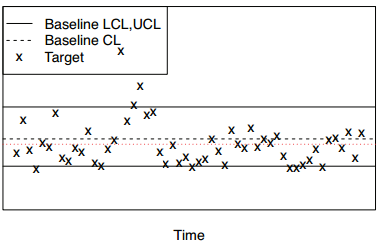
\includegraphics[scale=0.7]{Figures/controlchart.PNG}
\end{center}
  \caption{from ``Example of a control chart''\cite{nguyen2012using}}

\end{figure}


A control chart consists of a baseline data set (CL) and a target data set (Target). A baseline data set contains the results of the prior test. Based on this data set an upper (UCL) and lower limit (LCL) will be decided. The target data set contains the results of the new test.

From these two data sets the violation ratio can be calculated. This is the percentage of the amount of targets outside the upper and lower limit. If performance regression occurs, the violation ratio is too high. In figure 1 only a few targets are outside the upper and lower limit, so most probababely no regression has occured.

It now seems easy to detect if performance regression occurs: a certain threshold on the maximum allowed violation ratio can be chosen, and if the violation ratio is higher than this threshold, performance regression has occurred. Unfortunately, this is not the case. There are some reasons that make it hard to detect performance regression. If the violation ratio is low, the probability that performance regression has occurred is low as well. A high violation ratio doesn't always mean that performance regression has occurred. Some performance counters are inconsistent, and show different results on the same input data. Because of this, it is possible that the violation ratio is higher than the chosen threshold but no performance regression has occurred. To avoid this, the prior test will be executed again after the new test.

\section{Association rules}
Another way to filter the results of performance regression testing is by using association rules. An association rule has a premise and a consequent. A rule predicts the occurence of a consequent, based on a premise. Association rules can be derived from a frequent item set. ``A frequent item set describes a set of metrics that appear together frequently.''\cite{foo2010mining} To discover a frequent item set, the Apriori algorithm can be used. The Apriori algorithm uses support and confidence to reduce the amount of candiadte rules generated:
``Support is the frequency at which all items in an association rule are observed together''. \cite{foo2010mining}. If the support is low, the assocation should not be analyzed, but if the support is high it should. Confidence is the probability that the assocation rule's premise leads to the consequent and has a value between 0 and 1. If the value is 0, it means that the confidence has not changed for a new test, and if the value is 1 the confidence of a rule is totally different. A threshold is created to filter out the consequences of the rules that have changed to much.






